% Provenance (never printed): see sources/outline_sources.md (Year 2: metamorphic reactions,
% Clapeyron slopes, the Al2SiO5 diagram, the facies grid, protoliths). Definitions and facies
% table from the IUGS subcommission proposal (via the Granada translation); thermodynamic data
% from Robie and Hemingway (1995); experimental diagram from Holdaway and Mukhopadhyay (1993);
% curves from figdata/bachelor-2/facies.py; exercise and problem values in the Book 4 scratch
% calculator calc/ch10.py.
\chapter{Reações e fácies metamórficas}\label{ch:b2:metamorphic-facies}

Um basalto que afunda com sua placa não continua sendo um basalto. Seu plagioclásio e seu piroxênio
reagem, no estado sólido, formando outros minerais, e a nova assembleia depende da
pressão e da temperatura que ele atingiu: uma rocha azul de glaucofana e lawsonita, ou uma
rocha verde e vermelha de onfacita e granada. As rochas metamórficas conservam esses minerais quando
voltam à superfície, e um petrólogo que conhece as reações pode reconstituir as
condições. Este capítulo escreve essas reações com a termodinâmica do
curso de química, calcula a partir de dados medidos o mais célebre diagrama de fases metamórfico,
o dos três minerais \ce{Al2SiO5}, compara-o com os experimentos e organiza as
assembleias das rochas metamórficas em fácies.
% ledger: scmr:facies-assemblages

\begin{recall}
\textbf{Do volume do ensino médio}: \omterm{def:b2:metamorphic-facies:metamorphism}{metamorfismo}, grau metamórfico, minerais-índice
e isógradas, \omterm{def:b2:metamorphic-facies:metamorphism}{metamorfismo} de contato e sua auréola, foliação e xistosidade,
pressão litostática; cianita, andaluzita e silimanita como polimorfos, e seu
diagrama de fases. \textbf{Dos volumes do primeiro ano dos livros de física e de química}: a energia
de Gibbs $G = H - TS$, cujo mínimo marca o estado estável a $T$ e $P$ dados;
entalpia, entropia e capacidade térmica; $\mathrm dG = V\,\mathrm dP - S\,\mathrm dT$; a
relação de Clausius--Clapeyron para a vaporização de uma substância pura e o ponto
triplo da água. \textbf{Do volume do primeiro ano}: zonas de subducção, cinturões de colisão e
a geoterma.
\end{recall}

\section{O metamorfismo}\label{sec:b2:metamorphic-facies:metamorphism}

O volume do ensino médio apresentou o \omterm{def:b2:metamorphic-facies:metamorphism}{metamorfismo} como a transformação de uma rocha pelo calor e pela
pressão. Uma recomendação internacional dá a definição usada aqui.

\begin{definition}[Metamorfismo; protólito]\label{def:b2:metamorphic-facies:metamorphism}
O \emph{metamorfismo}\index{metamorfismo} é um processo que modifica os minerais ou a
microestrutura de uma rocha, ou ambos, essencialmente no estado sólido, à medida que a rocha se ajusta
a condições físicas diferentes daquelas sob as quais se formou e daquelas
normalmente encontradas na superfície da Terra e na zona da diagênese. Ele pode coexistir com
a \omterm{def:b2:mantle-melting:melting}{fusão parcial} e pode modificar a composição química da rocha. A rocha antes do
metamorfismo é seu \emph{protólito}\index{protólito}.
\end{definition}
% ledger: scmr:metamorphism

O limite inferior exclui a diagênese, as transformações de um sedimento à medida que é soterrado e
litificado, e o limite superior é a fusão, estudada no \cref{ch:b2:crustal-melting}. Os
agentes são a temperatura, a pressão, os fluidos que circulam pela rocha (água e
dióxido de carbono, sobretudo) e a deformação. O \omterm{def:b2:metamorphic-facies:metamorphism}{metamorfismo} é classificado por sua extensão e
por seu contexto.
% ledger: scmr:metamorphism, scmr:types

O \omterm{def:b2:metamorphic-facies:metamorphism}{metamorfismo} \emph{regional} afeta grandes volumes de rocha e acompanha processos tectônicos
de grande escala: é \emph{orogênico} nas cadeias de montanhas, onde a crosta se espessa em uma
colisão; o \omterm{def:b2:metamorphic-facies:metamorphism}{metamorfismo} \emph{de soterramento} afeta rochas profundamente soterradas sob espessas
pilhas sedimentares ou vulcânicas, sem deformação nem magmatismo, de modo que suas rochas
em geral não têm xistosidade; o \omterm{def:b2:metamorphic-facies:metamorphism}{metamorfismo} \emph{de fundo oceânico} altera a crosta perto
das dorsais em expansão, onde a água do mar quente circula através dela sob fortes gradientes
térmicos, e sua recristalização é em geral incompleta. O \omterm{def:b2:metamorphic-facies:metamorphism}{metamorfismo} \emph{local}
tem uma causa local: o \omterm{def:b2:metamorphic-facies:metamorphism}{metamorfismo} \emph{de contato} aquece as encaixantes de uma intrusão;
o \omterm{def:b2:metamorphic-facies:metamorphism}{metamorfismo} \emph{hidrotermal} é movido por fluidos quentes ricos em água;
o \omterm{def:b2:metamorphic-facies:metamorphism}{metamorfismo} \emph{de deslocamento}, em zonas de falha e de cisalhamento, reduz o tamanho dos grãos e
produz milonitos e cataclasitos; o \omterm{def:b2:metamorphic-facies:metamorphism}{metamorfismo} \emph{de impacto}, sob o impacto de um \omterm{def:b2:planet-formation-meteorites:fall-find}{meteorito},
pode fundir e vaporizar a rocha. O \omterm{def:b2:metamorphic-facies:metamorphism}{metamorfismo} é dito progressivo enquanto a temperatura sobe e
retrógrado enquanto ela desce.
% ledger: scmr:types

\section{As reações metamórficas}\label{sec:b2:metamorphic-facies:reactions}

\begin{definition}[Reação metamórfica; reação de desvolatilização]\label{def:b2:metamorphic-facies:reaction}
Uma \emph{reação metamórfica}\index{reação metamórfica} transforma um conjunto de minerais
de uma rocha, os reagentes, em outro conjunto, os produtos, no estado sólido, eventualmente
com a participação de uma fase fluida. Uma \emph{reação de desvolatilização}\index{reação de desvolatilização}
é uma reação que libera um volátil: água em uma reação de desidratação, ou dióxido
de carbono em uma reação de descarbonatação.
\end{definition}

Três tipos aparecerão neste capítulo. As mudanças polimórficas, como cianita em
silimanita ou calcita em aragonita, conservam a fórmula e mudam a estrutura.
Outras reações entre sólidos redistribuem componentes entre minerais, como a
albita dando jadeíta mais quartzo:
\[
\ce{NaAlSi3O8 -> NaAlSi2O6 + SiO2}.
\]
As \omterm{def:b2:metamorphic-facies:reaction}{reações de desvolatilização} liberam um fluido, como a muscovita e o quartzo que se decompõem
a alta temperatura:
\[
\ce{KAl3Si3O10(OH)2 + SiO2 -> KAlSi3O8 + Al2SiO5 + H2O}.
\]
% ledger: day73:ms-qz

Para uma reação entre minerais de composição fixa, a variação da energia de Gibbs é
$\Delta_r G(T, P) = \sum G_{\text{produtos}} - \sum G_{\text{reagentes}}$; os produtos
são estáveis onde $\Delta_r G < 0$, os reagentes onde $\Delta_r G > 0$, e os dois
coexistem onde $\Delta_r G = 0$.

\begin{definition}[Reação univariante]\label{def:b2:metamorphic-facies:univariant}
Uma reação entre fases de composição fixa é \emph{univariante}\index{reação univariante}
quando sua condição de equilíbrio $\Delta_r G(T, P) = 0$ deixa uma variável
livre: o equilíbrio é uma linha no plano pressão--temperatura, que separa
o campo dos reagentes do dos produtos.
\end{definition}

\begin{definition}[Inclinação de Clapeyron]\label{def:b2:metamorphic-facies:clapeyron}
A \emph{inclinação de Clapeyron}\index{inclinação de Clapeyron} de uma reação é a inclinação
$\mathrm dP/\mathrm dT$ de sua linha de equilíbrio no plano pressão--temperatura.
\end{definition}

\begin{proposition}[Inclinação de Clapeyron de uma reação]\label{prop:b2:metamorphic-facies:clapeyron}
Ao longo da linha de equilíbrio de uma reação de variação de entropia $\Delta_r S$ e de variação
de volume $\Delta_r V$,
\[
\frac{\mathrm dP}{\mathrm dT} = \frac{\Delta_r S}{\Delta_r V}.
\]
\end{proposition}

\begin{proof}
Para cada fase, $\mathrm dG = V\,\mathrm dP - S\,\mathrm dT$; logo, para a reação,
$\mathrm d(\Delta_r G) = \Delta_r V\,\mathrm dP - \Delta_r S\,\mathrm dT$. Ao longo da linha,
$\Delta_r G = 0$ permanece nulo: $\Delta_r V\,\mathrm dP = \Delta_r S\,\mathrm dT$.
\end{proof}

É a relação de Clausius--Clapeyron da física, escrita para sólidos. Com
$\Delta_r S$ em \unit{J.mol^{-1}.K^{-1}} e $\Delta_r V$ em \unit{J.bar^{-1}} (um
\unit{J.bar^{-1}} equivale a \qty{10}{cm^3}), a inclinação sai em bars por kelvin. Duas
consequências moldam todo diagrama de fases metamórfico. Entre sólidos, as variações de entropia e de volume
são pequenas, de modo que uma linha de reação pode ser íngreme ou suave, positiva ou
negativa: o lado de alta temperatura contém os produtos de maior entropia, e o
lado de alta pressão os de menor volume. Em uma \omterm{def:b2:metamorphic-facies:reaction}{reação de desvolatilização}, o fluido
traz uma grande entropia, de modo que os produtos ficam do lado de alta temperatura; e o volume
do fluido, grande a baixa pressão e diminuindo à medida que a pressão sobe, torna a inclinação
suave a baixa pressão e mais íngreme a alta pressão. A linha de reação se curva.
Os experimentos sobre muscovita e quartzo a situam em 603, 637 e \qty{662}{\celsius} a 1,
2 e \qty{3}{kbar} de pressão de água: entre 1 e \qty{2}{kbar}, a linha sobe
\qty{29}{bar} por kelvin; entre 2 e 3, \qty{40}{bar} (\cref{exo:b2:metamorphic-facies:9}).
% ledger: day73:ms-qz

\section{Os aluminossilicatos}\label{sec:b2:metamorphic-facies:al2sio5}

\begin{definition}[Polimorfos de aluminossilicato]\label{def:b2:metamorphic-facies:al2sio5}
Os \emph{polimorfos de aluminossilicato}\index{polimorfos de aluminossilicato} são os três
minerais de fórmula \ce{Al2SiO5}: cianita (triclínica), andaluzita e silimanita (ambas
ortorrômbicas).
\end{definition}
% ledger: rh95:al2sio5

Eles são comuns nos lamitos metamorfizados, cujo alumínio carregam, e, como
partilham uma fórmula, qual deles cresce depende apenas da pressão e da temperatura. A tabela
abaixo dá suas propriedades medidas.

\begin{center}
\small
\begin{tabular}{@{}lrrrr@{}}
\hline
 & $\Delta_f H^\circ$ (\unit{kJ.mol^{-1}}) & $S^\circ$ (\unit{J.mol^{-1}.K^{-1}}) & $V^\circ$ (\unit{J.bar^{-1}}) & densidade (\unit{g.cm^{-3}})\\
\hline
cianita & $-2593.8$ & 82.80 & 4.415 & 3.670\\
andaluzita & $-2589.9$ & 91.39 & 5.152 & 3.145\\
silimanita & $-2586.1$ & 95.40 & 4.986 & 3.250\\
\hline
\end{tabular}
\par\smallskip{\small Cianita, andaluzita e silimanita a \qty{298.15}{K} e
\qty{1}{bar} (Robie e Hemingway, 1995); as entalpias têm incerteza de
\qty{2.0}{kJ.mol^{-1}}, as entropias de 0.5. Densidade a partir da massa molar,
\qty{162.046}{g.mol^{-1}}, e do volume.}
\end{center}
% ledger: rh95:al2sio5

A cianita é a mais densa e tem a menor entropia: é o polimorfo de alta pressão e
baixa temperatura. A andaluzita, a menos densa, ocupa as baixas pressões; a silimanita,
de maior entropia, as altas temperaturas. Suas linhas de equilíbrio podem ser calculadas.

\begin{method}[Calcular uma linha de reação]\label{met:b2:metamorphic-facies:line}
(1) A partir das tabelas, forme $\Delta_r H$, $\Delta_r S$ e $\Delta_r V$ a \qty{298.15}{K}
e \qty{1}{bar}. (2) Despreze a variação de $\Delta_r H$ e $\Delta_r S$ com a
temperatura (capacidades térmicas de produtos e reagentes quase iguais) e a de $\Delta_r V$
com a pressão e a temperatura (os sólidos mal se comprimem ou se dilatam):
\[
\Delta_r G(T, P) \approx \Delta_r H - T\,\Delta_r S + \Delta_r V\,(P - 1).
\]
(3) Iguale-a a zero: $P = 1 + (T\,\Delta_r S - \Delta_r H)/\Delta_r V$, uma reta de
inclinação $\Delta_r S/\Delta_r V$. (4) Quando a precisão importa, substitua $\Delta_r H$ e
$\Delta_r S$ por seus valores à temperatura $T$, a partir de tabelas de $H_T - H_{298}$ e $S_T$,
e resolva de novo. (5) Conserve apenas a parte de cada linha em que suas duas fases são mais estáveis
que qualquer terceira.
\end{method}

Para cianita em andaluzita, $\Delta_r H = \qty{3.9}{kJ}$, $\Delta_r S =
\qty{8.59}{J.K^{-1}}$ e $\Delta_r V = \qty{0.737}{J.bar^{-1}}$: a \qty{25}{\celsius}
e \qty{1}{bar}, $\Delta_r G = 3900 - 298.15\times8.59 = \qty{+1.34}{kJ}$, de modo que a cianita,
e não a andaluzita, é o polimorfo estável na superfície da Terra; cianita em silimanita tem
ali $\Delta_r G = \qty{+3.94}{kJ}$. As inclinações são $8.59/0.737 = \qty{11.7}{bar/K}$ para
cianita em andaluzita, $12.60/0.571 = \qty{22.1}{bar/K}$ para cianita em silimanita e
$4.01/(-0.166) = \qty{-24.2}{bar/K}$ para andaluzita em silimanita, a única reação das
três cujo produto de alta temperatura é o mais denso.
% ledger: rh95:al2sio5

\begin{definition}[Ponto invariante]\label{def:b2:metamorphic-facies:invariant}
Um \emph{ponto invariante}\index{ponto invariante} é um ponto do
plano pressão--temperatura em que três ou mais fases de um sistema coexistem em
equilíbrio e todas as linhas \omterm{def:b2:metamorphic-facies:univariant}{univariantes} entre elas se encontram; nenhuma variável fica livre ali.
\end{definition}

\begin{proposition}[O ponto triplo]\label{prop:b2:metamorphic-facies:triple}
As três linhas cianita $=$ andaluzita, cianita $=$ silimanita e andaluzita $=$
silimanita se encontram em um ponto. Em torno dele, cada linha é estável de um só lado; seu
prolongamento metaestável fica no campo do terceiro polimorfo.
\end{proposition}

\begin{proof}
Para todo $(T, P)$, $\Delta G_{\text{ky}\to\text{sil}} = \Delta G_{\text{ky}\to\text{and}} +
\Delta G_{\text{and}\to\text{sil}}$, já que as energias de Gibbs da andaluzita se cancelam. Onde
as duas primeiras linhas se cruzam, dois desses termos se anulam, logo o terceiro também: a terceira
linha passa pelo cruzamento. Além do cruzamento, sobre a linha cianita $=$ andaluzita,
por exemplo, $G_{\text{ky}} = G_{\text{and}}$, mas o ponto fica do lado da silimanita das
duas outras linhas, de modo que $G_{\text{sil}}$ é menor que ambas: nem a cianita nem a andaluzita
é estável ali, e a linha é metaestável.
\end{proof}

Com as propriedades constantes do método, o ponto triplo fica a
\qty{514}{\celsius} e \qty{3.88}{kbar} (o problema de fim de semana); com a dependência
em temperatura das tabelas, a \qty{536}{\celsius} e \qty{4.20}{kbar}. O diagrama
experimental, construído a partir de experimentos reversos, situa-o a $504 \pm \qty{20}{\celsius}$ e
$3.75 \pm \qty{0.25}{kbar}$ (a figura abaixo).
% ledger: rh95:al2sio5-ht, hm93:triple, hm93:table11

\begin{omfigure}
\centering
\begin{tikzpicture}
\begin{axis}[omrecord, width=0.84\linewidth, height=7.4cm,
  xmin=200, xmax=900, ymin=0, ymax=10, xlabel={$T$ (\unit{\celsius})}, ylabel={$P$ (\unit{kbar})},
  legend style={font=\scriptsize, at={(0.02,0.98)}, anchor=north west},
  tick label style={font=\scriptsize}, label style={font=\small}]
\addplot[very thick, blue!70!black] table[x=T_C, y=P_kbar] {figdata/out/bachelor-2-facies-stable-kyand.dat};
\addlegendentry{calculado (tabelas)}
\addplot[thick, gray, densely dashed, mark=o, mark size=1.2pt] table[x=T_C, y=P_kbar] {figdata/out/bachelor-2-facies-hm93-kyand.dat};
\addlegendentry{experimental}
\addplot[thick, orange!85!black, mark=square*, mark size=1.3pt] table[x=T_C, y=P_kbar] {figdata/out/bachelor-2-facies-day73.dat};
\addlegendentry{muscovita + quartzo}
\addplot[very thick, blue!70!black, forget plot] table[x=T_C, y=P_kbar] {figdata/out/bachelor-2-facies-stable-kysil.dat};
\addplot[very thick, blue!70!black, forget plot] table[x=T_C, y=P_kbar] {figdata/out/bachelor-2-facies-stable-andsil.dat};
\addplot[thin, blue!70!black, dashed, forget plot] table[x=T_C, y=P_kbar] {figdata/out/bachelor-2-facies-meta-kyand.dat};
\addplot[thin, blue!70!black, dashed, forget plot] table[x=T_C, y=P_kbar] {figdata/out/bachelor-2-facies-meta-kysil.dat};
\addplot[thin, blue!70!black, dashed, forget plot] table[x=T_C, y=P_kbar] {figdata/out/bachelor-2-facies-meta-andsil.dat};
\addplot[thick, gray, densely dashed, mark=o, mark size=1.2pt, forget plot] table[x=T_C, y=P_kbar] {figdata/out/bachelor-2-facies-hm93-kysil.dat};
\addplot[thick, gray, densely dashed, mark=o, mark size=1.2pt, forget plot] table[x=T_C, y=P_kbar] {figdata/out/bachelor-2-facies-hm93-andsil.dat};
\addplot[only marks, mark=*, mark size=2pt, blue!70!black, forget plot] table[x=T_C, y=P_kbar] {figdata/out/bachelor-2-facies-triple-B.dat};
\addplot[only marks, mark=*, mark size=2pt, gray, forget plot] table[x=T_C, y=P_kbar] {figdata/out/bachelor-2-facies-hm93-triple.dat};
\node[font=\small\bfseries] at (axis cs:330,6.2) {cianita};
\node[font=\small\bfseries] at (axis cs:460,0.6) {andaluzita};
\node[font=\small\bfseries] at (axis cs:790,3.6) {silimanita};
\end{axis}
\end{tikzpicture}
\par\smallskip{\small O diagrama \ce{Al2SiO5} calculado a partir das tabelas termodinâmicas de
Robie e Hemingway (1995), com entalpia e entropia dependentes da temperatura (azul; tracejado:
prolongamentos metaestáveis), e o diagrama experimental de Holdaway e Mukhopadhyay (1993)
(cinza, seus pontos tabelados). Laranja: a decomposição de muscovita + quartzo medida por
Day (1973), que se curva.}
\end{omfigure}
% ledger: rh95:al2sio5, rh95:al2sio5-ht, hm93:table11, hm93:triple, day73:ms-qz

A linha cianita--andaluzita calculada fica a menos de \qty{0.1}{kbar} da linha experimental
entre 400 e \qty{600}{\celsius}, mas a linha andaluzita--silimanita fica
\qty{0.65}{kbar} alta demais a \qty{600}{\celsius}. Essa linha é a mais frágil das
três: com $\Delta_r V = \qty{-0.166}{J.bar^{-1}}$, um erro de \qty{0.1}{kJ} em
$\Delta_r H$, um vigésimo da incerteza de cada entalpia da tabela, desloca-a de
\qty{600}{bar}. As próprias entalpias das tabelas são ajustadas para reproduzir os
experimentos, dentro de suas incertezas; são os experimentos, e não a calorimetria sozinha, que fixam o
diagrama.
% ledger: rh95:al2sio5, hm93:adjusted, hm93:table11

A figura abaixo mostra por que uma linha é uma fronteira. A \qty{6}{kbar}, as energias de Gibbs da
andaluzita e da silimanita, medidas a partir da da cianita, cruzam o zero onde cada uma se
tornaria mais estável que a cianita; as diferenças nunca passam de alguns quilojoules por mol,
e é por isso que um pequeno erro em uma entalpia desloca tanto uma linha.

\begin{omfigure}
\centering
\begin{tikzpicture}
\begin{axis}[omrecord, width=0.7\linewidth, height=5.4cm,
  xmin=300, xmax=900, ymin=-4, ymax=4.5, xlabel={$T$ (\unit{\celsius})},
  ylabel={$G - G_{\text{cianita}}$ (\unit{kJ.mol^{-1}})},
  legend style={font=\scriptsize, at={(0.02,0.02)}, anchor=south west},
  tick label style={font=\scriptsize}, label style={font=\small}]
\addplot[very thick, red!75!black] table[x=T_C, y=dG_and] {figdata/out/bachelor-2-facies-dg6.dat};
\addlegendentry{andaluzita}
\addplot[very thick, green!45!black] table[x=T_C, y=dG_sil] {figdata/out/bachelor-2-facies-dg6.dat};
\addlegendentry{silimanita}
\addplot[thin, black] coordinates {(300,0) (900,0)};
\end{axis}
\end{tikzpicture}
\par\smallskip{\small Energias de Gibbs da andaluzita e da silimanita em relação à cianita a
\qty{6}{kbar}, a partir das mesmas tabelas. A cianita é estável enquanto as duas curvas são positivas;
a silimanita assume a partir de \qty{624}{\celsius}. A andaluzita só cruza o zero a
\qty{692}{\celsius}, onde a silimanita já está mais baixa: acima da pressão do
ponto triplo, a andaluzita nunca é a mais estável.}
\end{omfigure}
% ledger: rh95:al2sio5, rh95:al2sio5-ht

\begin{inthelab}[Reverter uma reação]
Uma linha de reação é localizada em laboratório por experimentos a pressão e
temperatura fixas que partem de uma mistura de reagentes e produtos. Em um aparelho
pistão--cilindro, a mistura é mantida de um a alguns dias; o sentido da reação é então
lido por difração de raios X, comparando a razão entre os picos do produto e do reagente
com a da mistura inicial, e confirmado por sobrecrescimentos no mineral estável. Outros
estudos pesam um único cristal de andaluzita que reagiu em um pó de cianita ou de
silimanita, com uma microbalança precisa a cerca de \qty{4}{\micro g}. Um equilíbrio é
\emph{revertido} quando se observou o crescimento de cada lado em um e no outro lado da linha;
a linha fica então no intervalo entre eles, traçado com os erros do aparelho,
tipicamente \qty{10}{\celsius} e \qty{0.5}{kbar}. Os experimentadores julgam um diagrama de fases primeiro
por essas reversões, e só depois pelas rochas.
\end{inthelab}
% ledger: hm93:methods

\section{Assembleias e fácies}\label{sec:b2:metamorphic-facies:facies}

\begin{definition}[Assembleia mineral]\label{def:b2:metamorphic-facies:assemblage}
Uma \emph{assembleia mineral}\index{assembleia mineral} é o conjunto de minerais que cresceram
juntos em equilíbrio em uma rocha metamórfica.
\end{definition}

Uma assembleia depende das condições do \omterm{def:b2:metamorphic-facies:metamorphism}{metamorfismo} e da composição da
rocha. Eskola, que introduziu o conceito de fácies em 1915, viu que rochas de mesma
composição têm a mesma assembleia sob as mesmas condições, e que as
assembleias de rochas diferentes mudam juntas quando as condições mudam; a
recomendação internacional conserva seu conceito.
% ledger: scmr:facies

\begin{definition}[Fácies metamórfica; grade de fácies]\label{def:b2:metamorphic-facies:facies}
Uma \emph{fácies metamórfica}\index{fácies metamórfica} é um conjunto de assembleias minerais
metamórficas, repetidamente associadas no tempo e no espaço, que mostram uma relação regular
entre a composição mineral e a composição química global, de tal modo que fácies diferentes
correspondem a condições metamórficas diferentes, sobretudo temperatura e pressão. As
fácies são nomeadas e definidas pelas assembleias das rochas de composição basáltica. Uma
\emph{grade de fácies}\index{grade de fácies} é o arranjo das fácies no
plano pressão--temperatura.
\end{definition}
% ledger: scmr:facies

A tabela abaixo lista dez fácies por seus minerais diagnósticos nos metabasaltos.

\begin{center}
\small
\begin{tabular}{@{}p{0.27\linewidth}p{0.66\linewidth}@{}}
\hline
fácies & minerais diagnósticos de um metabasalto\\
\hline
zeólita & zeólitas como laumontita e heulandita\\
prehnita--pumpellyita & prehnita + pumpellyita, prehnita + actinolita, pumpellyita + actinolita\\
xisto verde & actinolita + albita + clorita + epidoto\\
epidoto-anfibolito & hornblenda + albita + epidoto $\pm$ clorita\\
anfibolito & hornblenda + plagioclásio (mais de \qty{17}{\percent} de anortita)\\
granulito & clinopiroxênio + ortopiroxênio + plagioclásio; olivina instável com plagioclásio ou granada\\
xisto azul & glaucofana + epidoto $\pm$ granada, ou glaucofana + lawsonita\\
eclogito & onfacita + granada; plagioclásio instável\\
\omterm{def:b2:magma-emplacement:aureole}{piroxênio-hornfels} & clinopiroxênio + ortopiroxênio + plagioclásio; olivina estável com plagioclásio\\
sanidinito & o mesmo, com minerais de temperatura muito alta, como a pigeonita\\
\hline
\end{tabular}
\par\smallskip{\small As fácies e suas assembleias diagnósticas nas rochas de composição
basáltica, segundo a recomendação internacional (as oito fácies de Eskola, com as fácies
zeólita e prehnita--pumpellyita acrescentadas depois).}
\end{center}
% ledger: scmr:facies-assemblages, scmr:facies

A recomendação insiste no que as fácies não fazem: elas registram regularidades entre
assembleias, e não procuram fixar a pressão e a temperatura de cada uma. Sua ordem no
plano pressão--temperatura decorre das reações entre elas, e a
figura abaixo a desenha esquematicamente. A temperatura cresce da fácies zeólita, passando
pelas fácies xisto verde e anfibolito, até a fácies granulito; a baixa pressão e alta
temperatura ficam as fácies \omterm{def:b2:magma-emplacement:aureole}{hornfels} das \omterm{def:b2:magma-emplacement:aureole}{auréolas de contato}; a alta pressão e baixa
temperatura, a fácies xisto azul; a alta pressão e temperatura mais alta, a
fácies eclogito. Reações deste capítulo fixam trechos das fronteiras: o plagioclásio,
presente como albita ou como um plagioclásio mais cálcico da fácies xisto verde à fácies
granulito, não é estável na fácies eclogito, como mostra sua
albita ao se transformar em jadeíta e quartzo (\cref{exo:b2:metamorphic-facies:8}); a calcita se transforma na
aragonita, mais densa, a alta pressão (\cref{exo:b2:metamorphic-facies:7}).
% ledger: scmr:facies, scmr:facies-assemblages

\begin{omfigure}
\centering
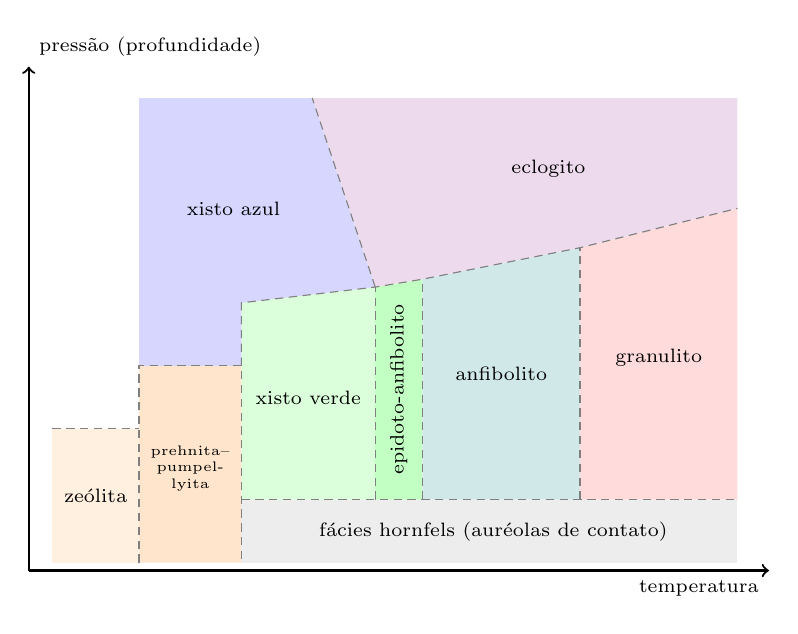
\begin{tikzpicture}[font=\scriptsize, x=1cm, y=1cm]
\draw[->, thick] (0,0) -- (9.4,0) node[below left] {temperatura};
\draw[->, thick] (0,0) -- (0,6.4) node[above right] {pressão (profundidade)};
\fill[orange!12] (0.3,0.1) -- (1.4,0.1) -- (1.4,1.8) -- (0.3,1.8) -- cycle;
\fill[orange!20] (1.4,0.1) -- (2.7,0.1) -- (2.7,2.6) -- (1.4,2.6) -- (1.4,1.8) -- cycle;
\fill[green!14] (2.7,0.9) -- (4.4,0.9) -- (4.4,3.6) -- (2.7,3.4) -- cycle;
\fill[green!24] (4.4,0.9) -- (5.0,0.9) -- (5.0,3.7) -- (4.4,3.6) -- cycle;
\fill[teal!18] (5.0,0.9) -- (7.0,0.9) -- (7.0,4.1) -- (5.0,3.7) -- cycle;
\fill[red!14] (7.0,0.9) -- (9.0,0.9) -- (9.0,4.6) -- (7.0,4.1) -- cycle;
\fill[gray!14] (2.7,0.1) -- (9.0,0.1) -- (9.0,0.9) -- (2.7,0.9) -- cycle;
\fill[blue!16] (1.4,2.6) -- (2.7,2.6) -- (2.7,3.4) -- (4.4,3.6) -- (3.6,6.0) -- (1.4,6.0) -- cycle;
\fill[violet!14] (4.4,3.6) -- (5.0,3.7) -- (7.0,4.1) -- (9.0,4.6) -- (9.0,6.0) -- (3.6,6.0) -- cycle;
\draw[gray, densely dashed] (1.4,0.1) -- (1.4,2.6) -- (2.7,2.6) -- (2.7,0.1);
\draw[gray, densely dashed] (0.3,1.8) -- (1.4,1.8);
\draw[gray, densely dashed] (2.7,0.9) -- (9.0,0.9);
\draw[gray, densely dashed] (4.4,0.9) -- (4.4,3.6) (5.0,0.9) -- (5.0,3.7) (7.0,0.9) -- (7.0,4.1);
\draw[gray, densely dashed] (2.7,2.6) -- (2.7,3.4) -- (4.4,3.6) -- (5.0,3.7) -- (7.0,4.1) -- (9.0,4.6);
\draw[gray, densely dashed] (4.4,3.6) -- (3.6,6.0);
\node at (0.85,0.95) {zeólita};
\node[align=center, font=\tiny] at (2.05,1.3) {prehnita--\\pumpel-\\lyita};
\node at (3.55,2.2) {xisto verde};
\node[rotate=90] at (4.7,2.3) {epidoto-anfibolito};
\node at (6.0,2.5) {anfibolito};
\node at (8.0,2.7) {granulito};
\node at (5.9,0.5) {fácies hornfels (auréolas de contato)};
\node at (2.6,4.6) {xisto azul};
\node at (6.6,5.1) {eclogito};
\end{tikzpicture}
\par\smallskip{\small A \omterm{def:b2:metamorphic-facies:facies}{grade de fácies}, esquemática: a ordem das fácies da tabela no
plano pressão--temperatura. As fronteiras são graduais e desenhadas sem números de
propósito: as fácies são definidas por assembleias, e as reações que as limitam dependem
da composição de cada rocha.}
\end{omfigure}
% ledger: scmr:facies, scmr:facies-assemblages

\begin{omfigure}
\centering
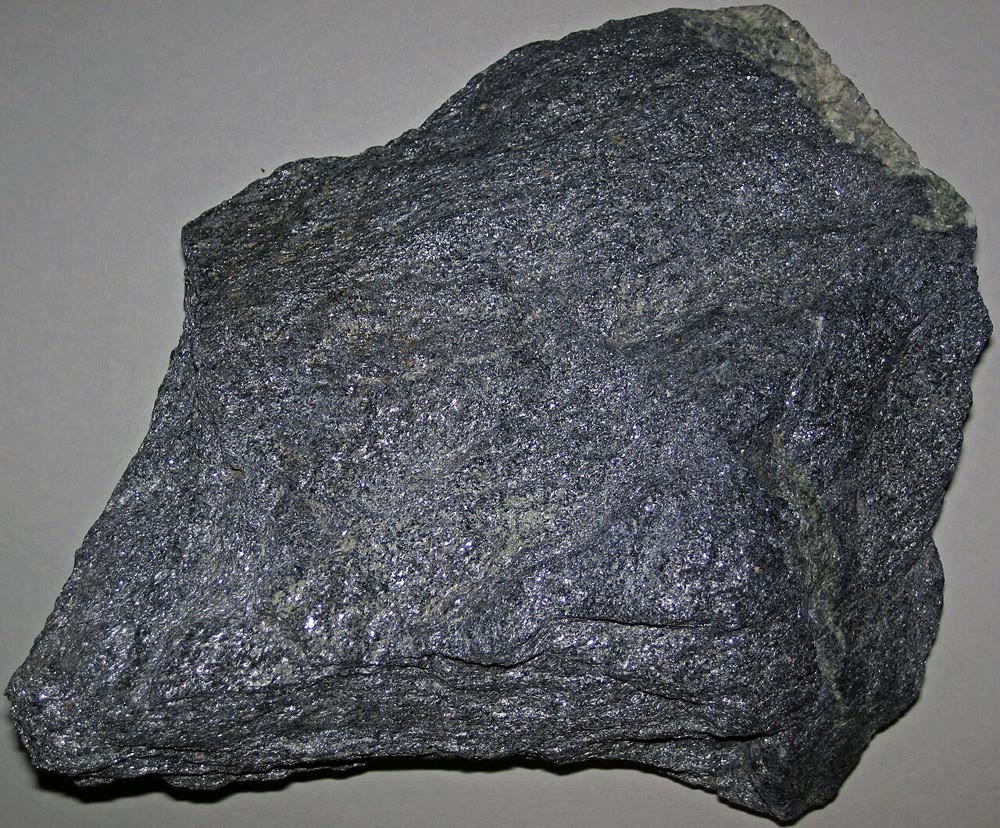
\includegraphics[width=0.27\linewidth]{images/book4/b2-10-blueschist.jpg}\hspace{0.02\linewidth}%
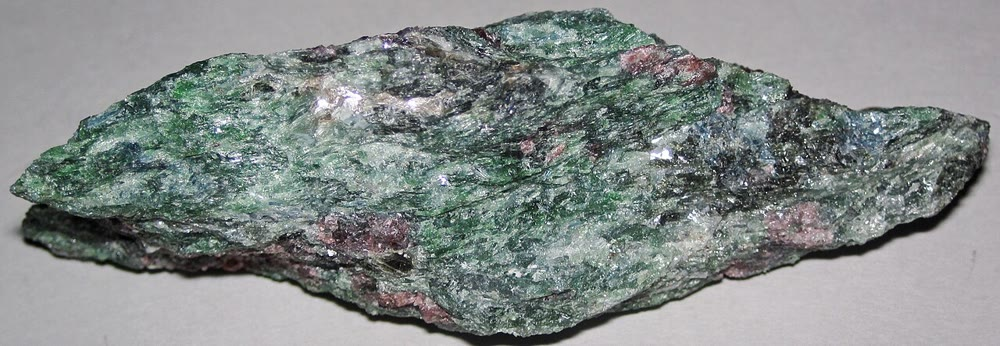
\includegraphics[width=0.69\linewidth]{images/book4/b2-10-eclogite.jpg}
\par\smallskip{\small Dois basaltos metamorfizados. À esquerda: um xisto azul com lawsonita do
Complexo Franciscano da Califórnia, azul de glaucofana. À direita: um eclogito do oeste da
Noruega, onfacita verde e granada vermelha com um pouco de quartzo, cianita e rutilo. Fotografias de
James St.~John, CC BY 2.0.}
\end{omfigure}

Rochas soterradas e aquecidas juntas passam pelas fácies em uma ordem regular, que
reflete a razão entre pressão e temperatura ao longo de sua trajetória: alta em uma zona de
subducção, onde se formam os xistos azuis; intermediária em um cinturão de colisão; baixa perto de uma intrusão.
O \cref{ch:b2:pt-paths} nomeia essas séries e lê essas trajetórias a partir dos minerais.
% ledger: scmr:facies

\section{O protólito importa}\label{sec:b2:metamorphic-facies:protoliths}

As fácies são definidas sobre basaltos, mas todo \omterm{def:b2:metamorphic-facies:metamorphism}{protólito} registra as mesmas condições em
seus próprios minerais.

\begin{definition}[Metapelito; metabasito]\label{def:b2:metamorphic-facies:protoliths}
Um \emph{metapelito}\index{metapelito} é um lamito metamorfizado (um pelito), rico em
alumínio e potássio, cujas assembleias contêm micas, clorita, granada, estaurolita e
os aluminossilicatos. Um \emph{metabasito}\index{metabasito} é um basalto,
gabro ou outra rocha máfica metamorfizada, rica em cálcio, magnésio e ferro, cujas assembleias definem
as fácies.
\end{definition}

Em um \omterm{def:b2:metamorphic-facies:protoliths}{metapelito}, os minerais-índice do volume do ensino médio aparecem em sequência à medida que
o grau aumenta (clorita, biotita, granada, estaurolita, cianita, silimanita), a
reação muscovita + quartzo deste capítulo produz silimanita e feldspato potássico a temperatura
ainda mais alta, e o aluminossilicato presente indica de que lado do ponto
triplo a rocha passou. Um calcário ou um dolomito metamorfizado torna-se um mármore, de calcita ou de
dolomita; os carbonatos impuros, com sílica e argila, tornam-se rochas calcissilicáticas cujas
reações de descarbonatação liberam dióxido de carbono; um arenito quartzoso torna-se um quartzito,
que mostra pouco além do tamanho de seus grãos. Um \omterm{def:b2:metamorphic-facies:protoliths}{metapelito} da zona da clorita e um
metabasalto ao lado dele, à mesma pressão e temperatura, não se parecem em nada, o
segundo uma rocha verde de actinolita, clorita, epidoto e albita: um só conjunto de condições,
duas assembleias.
% ledger: iugs:barrow, day73:ms-qz, scmr:facies-assemblages

\section{Exercícios}

\begin{exercise}[$\star$]\label{exo:b2:metamorphic-facies:1}
Dê o tipo de \omterm{def:b2:metamorphic-facies:metamorphism}{metamorfismo}: (a) um calcário recristalizado em mármore a menos de
\qty{500}{m} de um granito; (b) uma rocha de granulação fina, bandada, ao longo de uma grande falha
transcorrente, com os grãos esmagados e recristalizados; (c) um basalto da crosta oceânica cujo
vidro se transformou em clorita e zeólitas perto de uma dorsal, com seus minerais apenas parcialmente
substituídos; (d) arenitos vulcânicos na base de uma pilha de \qty{10}{km} de espessura,
recristalizados sem xistosidade.
\end{exercise}
% ledger: scmr:types

\begin{exercise}[$\star$]\label{exo:b2:metamorphic-facies:2}
A partir da tabela dos aluminossilicatos, calcule $\Delta_r S$, $\Delta_r V$ e a
\omterm{def:b2:metamorphic-facies:clapeyron}{inclinação de Clapeyron} de cianita $\to$ silimanita, em \unit{bar/K} e em \unit{MPa/K}. De quanto
varia a pressão de equilíbrio em \qty{100}{\celsius}?
\end{exercise}
% ledger: rh95:al2sio5

\begin{exercise}[$\star$]\label{exo:b2:metamorphic-facies:3}
A que fácies pertence cada metabasalto? (a) actinolita, albita, clorita e
epidoto; (b) glaucofana e lawsonita; (c) hornblenda e plagioclásio com
\qty{30}{\percent} de anortita; (d) onfacita e granada, sem plagioclásio.
\end{exercise}
% ledger: scmr:facies-assemblages

\begin{exercise}[$\star$]\label{exo:b2:metamorphic-facies:4}
(a) A partir da massa molar \qty{162.046}{g.mol^{-1}} e dos volumes molares 44.15, 51.52 e
\qty{49.86}{cm^3.mol^{-1}}, calcule as densidades da cianita, da andaluzita e da silimanita.
(b) Qual delas a pressão favorece, e por quê? (c) As bases de dados mineralógicas dão 3.61, 3.15 e
\qty{3.24}{g.cm^{-3}}: por que os cristais naturais podem diferir das fases puras?
\end{exercise}
% ledger: rh95:al2sio5, webmineral:polymorphs

\begin{exercise}[$\star\star$]\label{exo:b2:metamorphic-facies:5}
Para cianita $\to$ andaluzita, $\Delta_r H = \qty{3.9}{kJ}$, $\Delta_r S =
\qty{8.59}{J.K^{-1}}$, $\Delta_r V = \qty{0.737}{J.bar^{-1}}$. (a) Que polimorfo é
estável a \qty{25}{\celsius} e \qty{1}{bar}? (b) A que temperatura os dois
coexistem a \qty{1}{bar}? (c) Calcule a pressão de equilíbrio a \qty{400}{\celsius} e
compare-a com os \qty{2.54}{kbar} experimentais. (d) Por que, ainda assim, se encontra andaluzita
em rochas que se resfriaram até a superfície?
\end{exercise}
% ledger: rh95:al2sio5, hm93:table11

\begin{exercise}[$\star\star$]\label{exo:b2:metamorphic-facies:6}
Teste a etapa (2) do método. A \qty{1000}{K}, as tabelas dão $S_T$ = 285.02 para a cianita
e 296.44 para a silimanita, e $(H_T - H_{298})/T$ = 122.29 e 121.39
(\unit{J.mol^{-1}.K^{-1}}). (a) Calcule $\Delta_r H$, $\Delta_r S$ e $\Delta_r G$ de
cianita $\to$ silimanita a \qty{1000}{K} e \qty{1}{bar}. (b) Compare com os valores
constantes da tabela. (c) Que polimorfo é estável ali, e qual é o tamanho do erro do
método simples?
\end{exercise}
% ledger: rh95:al2sio5-ht, rh95:al2sio5

\begin{exercise}[$\star\star$]\label{exo:b2:metamorphic-facies:7}
A calcita e a aragonita (\ce{CaCO3}) têm, a \qty{298.15}{K}, $\Delta_f G$ = $-1128.5$ e
$-1127.4$ \unit{kJ.mol^{-1}}, $S$ = 91.7 e 88.0 \unit{J.mol^{-1}.K^{-1}}, $V$ = 36.93
e \qty{34.15}{cm^3.mol^{-1}}, e entalpias de formação iguais. (a) Encontre a
pressão de equilíbrio a \qty{25}{\celsius}. (b) Calcule a \omterm{def:b2:metamorphic-facies:clapeyron}{inclinação de Clapeyron}. (c) Encontre a
pressão de equilíbrio a \qty{300}{\celsius}. (d) Muitas conchas são feitas de aragonita e
vivem a \qty{1}{bar}: o que isso diz?
\end{exercise}
% ledger: rh95:cc-ar

\begin{exercise}[$\star\star$]\label{exo:b2:metamorphic-facies:8}
Para albita $\to$ jadeíta + quartzo, as tabelas dão $\Delta_r H = \qty{-5.0}{kJ}$,
$\Delta_r S = \qty{-32.4}{J.K^{-1}}$, $\Delta_r V = \qty{-1.698}{J.bar^{-1}}$. (a)
Calcule a \omterm{def:b2:metamorphic-facies:clapeyron}{inclinação de Clapeyron}. (b) Calcule a pressão de equilíbrio a \qty{500}{\celsius}.
(c) As entalpias de formação da albita, da jadeíta e do quartzo têm incertezas de 2.6, 3.6
e \qty{1.0}{kJ.mol^{-1}}; combinando-as como erros independentes, qual é a incerteza dessa
pressão? (d) Por que a fácies eclogito não tem plagioclásio?
\end{exercise}
% ledger: rh95:ab-jd-qz, scmr:facies-assemblages

\begin{exercise}[$\star\star$]\label{exo:b2:metamorphic-facies:9}
Muscovita + quartzo se decompõe a 603, 637 e \qty{662}{\celsius} a 1, 2 e
\qty{3}{kbar}. (a) Calcule a inclinação da linha entre cada par de pontos. (b) Se a
entropia de reação quase não varia nesse intervalo, por que fator $\Delta_r V$
diminuiu do primeiro intervalo para o segundo? (c) Que fase é responsável?
\end{exercise}
% ledger: day73:ms-qz

\begin{exercise}[$\star\star\star$]\label{exo:b2:metamorphic-facies:10}
Com as propriedades constantes do método: (a) calcule as pressões das três
reações a \qty{600}{\celsius}; (b) mostre que, a \qty{600}{\celsius} e à pressão de
cianita $=$ andaluzita, a silimanita é o polimorfo mais estável, de modo que esse ponto da
linha é metaestável; (c) que polimorfo é estável a \qty{600}{\celsius} e
\qty{4}{kbar}, e a \qty{600}{\celsius} e \qty{7}{kbar}?
\end{exercise}
% ledger: rh95:al2sio5

\begin{exercise}[$\star\star\star$]\label{exo:b2:metamorphic-facies:11}
Um xisto contém cianita, andaluzita e silimanita juntas, as três crescidas em
equilíbrio. (a) Com o ponto triplo experimental, $504 \pm \qty{20}{\celsius}$ e
$3.75 \pm \qty{0.25}{kbar}$, e uma crosta de densidade \qty{2700}{kg.m^{-3}} ($g =
\qty{9.81}{m.s^{-2}}$), a que profundidade ele cresceu? (b) Tomando \qty{10}{\celsius} na
superfície, que gradiente térmico médio isso implica? (c) Por que essas rochas são raras?
\end{exercise}
% ledger: hm93:triple

\begin{exercise}[$\star\star\star$]\label{exo:b2:metamorphic-facies:12}
Duas rochas são soterradas até a profundidade $z$, a partir de \qty{10}{\celsius} na superfície: a rocha X ao longo de
\qty{10}{\celsius.km^{-1}} até \qty{30}{km} sob rochas de densidade média
\qty{3000}{kg.m^{-3}}, a rocha Y ao longo de \qty{30}{\celsius.km^{-1}} até \qty{20}{km} sob rochas
de densidade média \qty{2800}{kg.m^{-3}}. (a) Calcule $T$ e $P$ no fim de cada trajetória.
(b) Com as linhas de propriedades constantes (calcita $=$ aragonita: $P = 13.31\,T$ bar com $T$
em kelvin; albita $=$ jadeíta + quartzo do \cref{exo:b2:metamorphic-facies:8}; os aluminossilicatos da
tabela), qual entre aragonita e calcita, entre jadeíta + quartzo e albita, e que
aluminossilicato contém cada rocha? (c) Que trajetória é a fria, de alta pressão, e em que fácies termina cada uma?
\end{exercise}
% ledger: rh95:cc-ar, rh95:ab-jd-qz, rh95:al2sio5

\section{Problema: construir o ponto triplo}

\begin{problem}[{Problema de fim de semana --- o diagrama dos aluminossilicatos a partir das tabelas, e até que
ponto confiar nele}]
\label{pb:b2:metamorphic-facies:1}
Use a tabela dos aluminossilicatos (\qty{298.15}{K}, \qty{1}{bar}) e o método deste
capítulo, com $\Delta_r H$, $\Delta_r S$ e $\Delta_r V$ constantes; escreva $T$ em
kelvin, $P$ em bar, e despreze o 1 em $P - 1$.

\noindent\textbf{Parte I --- As reações.}
\begin{enumerate}
\item Calcule $\Delta_r H$, $\Delta_r S$ e $\Delta_r V$ para cianita $\to$ andaluzita.
\item Faça o mesmo para cianita $\to$ silimanita.
\item Faça o mesmo para andaluzita $\to$ silimanita, e verifique que cada propriedade é a
diferença das duas primeiras.
\item Que polimorfo tem a maior entropia, qual o menor volume? De que lado
de cada linha ficará cada um?
\item Calcule as três \omterm{def:b2:metamorphic-facies:clapeyron}{inclinações de Clapeyron}.
\item Por que a inclinação de andaluzita $\to$ silimanita é negativa?
\end{enumerate}

\noindent\textbf{Parte II --- Por onde passam as linhas.}
\begin{enumerate}[resume]
\item Calcule $\Delta_r G$ das duas primeiras reações a \qty{298.15}{K}. Que
polimorfo é estável na superfície?
\item A que temperatura (em \unit{\celsius}) cada reação atinge o equilíbrio a
\qty{1}{bar}?
\item Das três temperaturas da questão~8, quais são equilíbrios estáveis e quais
metaestáveis? (Use a ordem das três a \qty{1}{bar}.)
\item Calcule a pressão de cianita $=$ andaluzita a \qty{400}{\celsius}; os
experimentos dão \qty{2.54}{kbar}.
\item Calcule a pressão de cianita $=$ silimanita a \qty{700}{\celsius}; os
experimentos dão \qty{7.86}{kbar}.
\item Esboce as três linhas entre 200 e \qty{900}{\celsius}.
\end{enumerate}

\noindent\textbf{Parte III --- O ponto triplo.}
\begin{enumerate}[resume]
\item Escreva as duas primeiras linhas como $P = a_i T - b_i$; dê $a_1$, $b_1$, $a_2$, $b_2$.
\item Resolva para a temperatura de sua interseção.
\item Calcule sua pressão.
\item Verifique que andaluzita $=$ silimanita passa por ela.
\item Compare com os valores experimentais $504 \pm \qty{20}{\celsius}$ e $3.75 \pm
\qty{0.25}{kbar}$.
\item Com a dependência em temperatura das tabelas, o ponto triplo se desloca para
\qty{536}{\celsius} e \qty{4.20}{kbar}. O refinamento o aproximou do
experimento? O que isso sugere sobre a principal fonte de erro?
\end{enumerate}

\noindent\textbf{Parte IV --- Até que ponto confiar nele.}
\begin{enumerate}[resume]
\item Aumente a entalpia de formação da andaluzita em \qty{1}{kJ}. De quanto
a linha cianita $=$ andaluzita se desloca em pressão, a temperatura fixa?
\item De quanto o ponto triplo se desloca em temperatura?
\item Faça o mesmo para um aumento de \qty{1}{kJ} na entalpia da silimanita.
\item Cada entalpia tem incerteza de \qty{2.0}{kJ}. Que intervalo de temperaturas do ponto
triplo os dados calorimétricos sozinhos permitem?
\item Como, então, as tabelas termodinâmicas podem reproduzir o diagrama experimental a menos de
\qty{30}{\celsius}?
\item Indique a temperatura do ponto triplo calculada na Parte III, arredondada ao
grau: o número-chave deste problema.
\end{enumerate}
\end{problem}
% ledger: rh95:al2sio5, rh95:al2sio5-ht, hm93:triple, hm93:table11, hm93:adjusted
